\documentclass[paper=8.27in:11.69in, 14pt, DIV=calc]{scrartcl}
\usepackage{geometry}
\usepackage{tikz}
\usepackage{graphicx}
\usepackage{pdfpages}
\usepackage{hyperref}
\usepackage{enumitem}
\usepackage{amsmath}
\newcounter{numbers}
\newcommand\printnumbers{\refstepcounter{numbers}\thenumbers}
\newcounter{answers}
\newcommand\printanswers{\refstepcounter{answers}\theanswers}


\begin{document}

\textbf{\begin{center}
\begin{Large}
CSCI 6315 Applied Database Systems\\
ASSIGNMENT 4: Data Storage and Querying, Transaction Management\\
Due is 04/28/2020 00:00\\
Ulvi Bajarani\\
Student ID 20539914\\
E-mail: ulvi.bajarani01@utrgv.edu\\
\end{Large}
\end{center}}

\newpage

\noindent \begin{center}
\textbf{Questions and Answers:}
\end{center}

\textbf{Problem \printnumbers . This problem has two parts:}

\begin{enumerate}[label=\alph*.]

\item Construct a $B^{+}$-tree for the following key values:\\
\\
2, 3, 5, 7, 11, 17, 19, 23, 29, 31.\\
\\
Assume that the number of pointers that will fit in one internal node is 4 and each leaf node can store 3 key values.\\

\item After the $B^{+}$-tree is constructed for Part a, show the final tree after the following operations:

\begin{enumerate}[label=\arabic*.]

\item Insert 9
\item Insert 10
\item Insert 8
\item Delete 23
\item Delete 19

\end{enumerate}

\textbf{Answer \printanswers. \\}

\begin{enumerate}[label=\alph*.]

\item \textbf{\textit{Assuming that nodes might contain 4 pointers (3 keys), the $B^{+}$ Tree is:\\}}

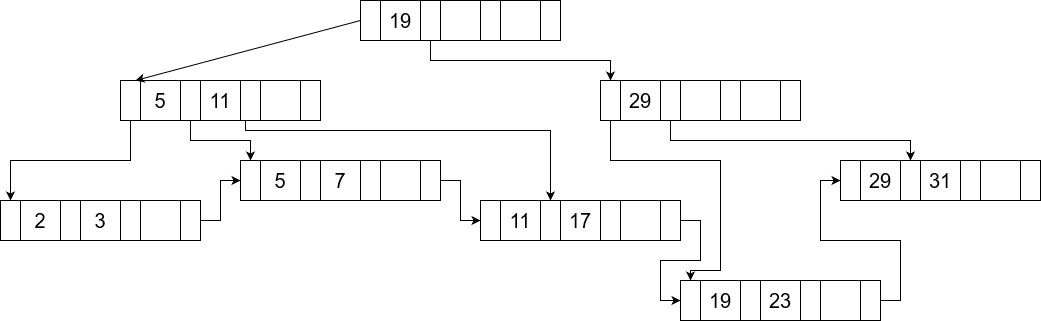
\includegraphics[scale=0.5]{InitialBPlus.png}

\begin{enumerate}[label=b.\arabic*.]

\item \textbf{After 9 insertion:}

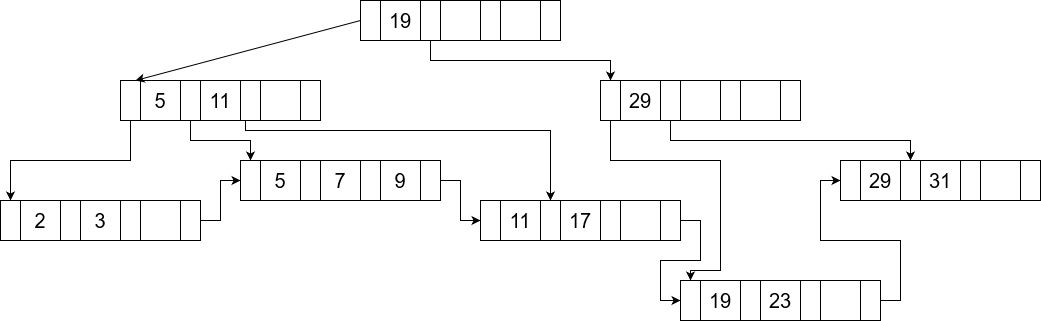
\includegraphics[scale=0.5]{After9Insertion.png}

\item \textbf{After 10 insertion:}

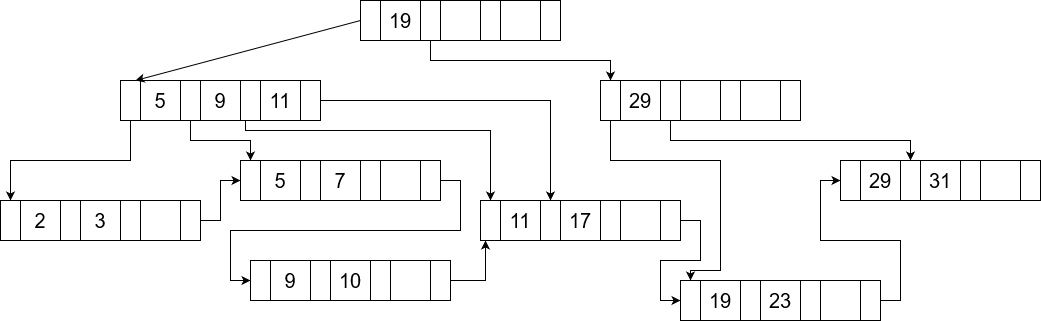
\includegraphics[scale=0.5]{After10Insertion.png}

\item \textbf{After 8 insertion:}

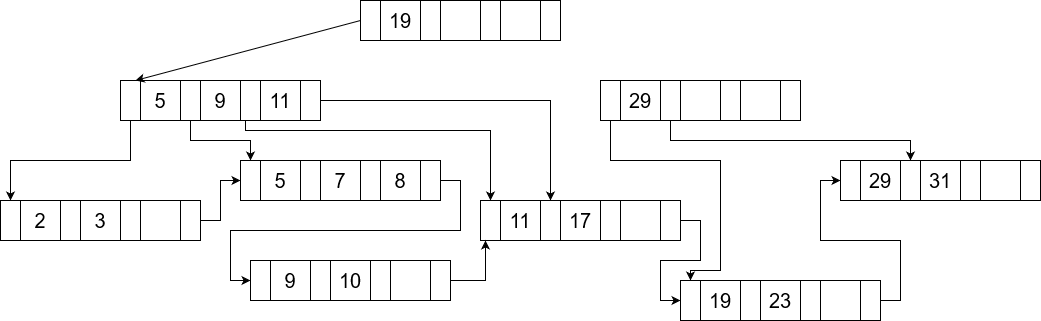
\includegraphics[scale=0.5]{After8Insertion.png}

\item \textbf{After 23 deletion:}

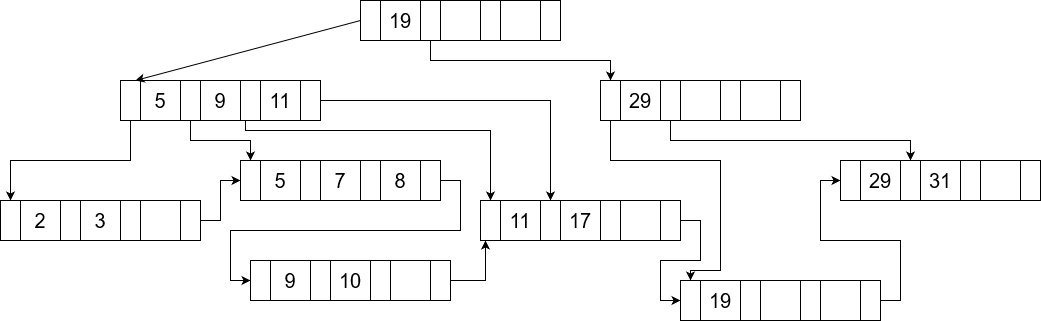
\includegraphics[scale=0.5]{After23Deletion.png}

\item \textbf{After 19 deletion. The final version:}

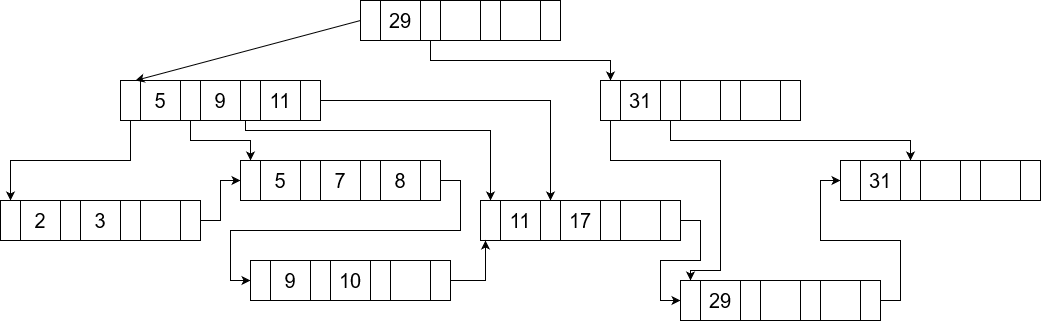
\includegraphics[scale=0.5]{After19Deletion.png}

\end{enumerate}

\end{enumerate}

\textbf{Problem \printnumbers . This problem has two parts:}

\end{enumerate}

\begin{enumerate}[label=\alph*.]

\item Suppose that we are using extendable hashing on a file that contains records with the following search key values:\\
\\
2, 3, 5, 7, 11, 17, 19, 23, 29, 31.\\
\\
Show the extendable hash structure for this file if the hash function is $ h(x) \ = \ x \ \% \ 8 $ and each bucket can hold three records.\\

\item After Completing Part a, show the extendable hash structures after the following operations:\\

\end{enumerate}

\begin{enumerate}[label=b.\arabic*.]

\item Delete 11
\item Delete 31
\item Insert 1
\item Insert 15

\end{enumerate}

\textbf{Answer \printanswers .\\}

\begin{enumerate}[label=\alph*.]

\item Since that we don't have the size in the description, I'll assume that there are two values initially (0 for 0 and even mods and 1 for odd mods). After the extensions, then table should look like this:

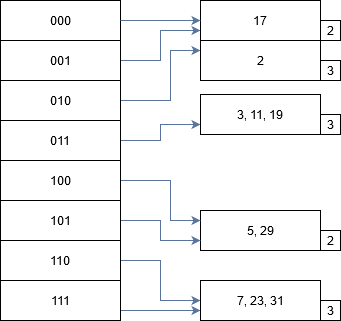
\includegraphics[]{ExHashTable.png}

\begin{enumerate}[label=b.\arabic*.]

\item \textbf{After 11 deletion:}

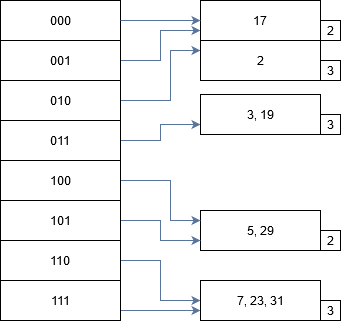
\includegraphics[]{ExHashTableAfter11Deletion.png}

\item \textbf{After 31 deletion:}

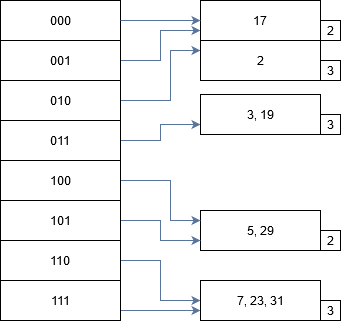
\includegraphics[]{ExHashTableAfter11Deletion.png}

\item \textbf{After 1 insertion:}

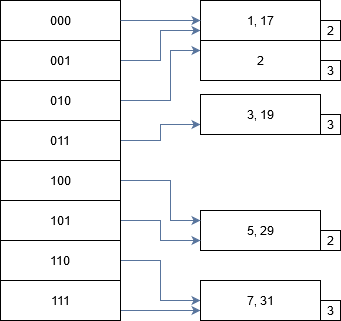
\includegraphics[]{ExHashTableAfter1Insertion.png}

\item \textbf{After 15 insertion. The final version:}

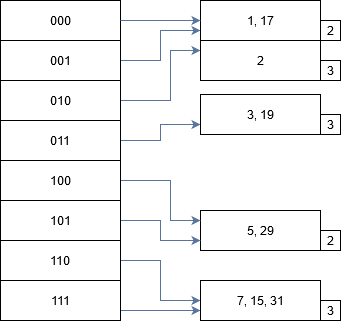
\includegraphics[]{ExHashTableAfter15Insertion.png}

\end{enumerate}

\end{enumerate}

\textbf{Problem \printnumbers . Consider the following SQL query for our University Database:\\
\\}
\textit{select T.dept\_name\\}
\textit{from department as T, department as S\\}
\textit{where T.budget $>$ S.budget and S.building = ``MAG"\\}
\\
Write an efficient relational-algebra expression that is equivalent to this query. Justify your choice.\\

\textbf{Answer \printanswers .\\}

$\Pi_{T.dept\_name}( (\Pi_{building, \ budget}(\rho_{_{T}}(department) ) ) ) \bowtie_{T.budget \ > \ S.budget} (\Pi_{budget}(\sigma_{(S.building = ``MAG")}(\rho_{_{S}}(department) ) ) )$\\
\\

The expression is efficient due to these reasons:

\begin{enumerate}[label=b.\arabic*.]

\item The expression performs the theta-join on the smallest possible amount of data, because of the restriction the right-hand side of the join to only the branches in ``MAG".

\item The expression eliminates the unnecessary attributes from both sides of the theta-join operation, e.g. from both the operands.

\end{enumerate}

\textbf{Problem \printnumbers . Let the relations $r_{1}(A, \ B, \ C)$ and $r_{2}(C, \ D, \ E)$ have the following properties: $r_{1}$ has 20,000 tuples, $r_{2}$ has 45,000 tuples, 25 tuples of $r_{1}$ fit on one block, and 30 tuples of $r_{2}$ fit on one block.} Estimate the number of block accesses required, using each of the following join strategies for $r_{1} \ \bowtie \ r_{2}$\\

\begin{enumerate}[label=\alph*.]

\item Nested-loop join
\item Block nested-loop join
\item Merge join
\item Hash join

\end{enumerate}

\textbf{Answer \printanswers .\\}

\noindent r1 = 20000 tuples\\
r2 = 45000 tuples\\
25 tuples of $r_{1}$ fit on one block\\
30 tuples of $r_{2}$ fit on one block\\

\noindent$b{r_{1}}$ = Number of blocks for $r_{1}$ is 20000/25=800\\
$b{r_{2}}$ = Number of blocks for $r_{2}$ is 45000/30=1500

\begin{enumerate}[label=\alph*.]

\item In the worst case,

$b{r_{1}} + r_{1} = 800 + 20000 = 20800$ seeks

$n{r_{1}} * b{r_{2}} + b{r_{1}} = 20000 * 1500 + 800 = 30000800$ block transfers.

Total disk accesses = $30000800 + 20800 = 30021600$

or

$b{r_{2}} + r_{2} = 1500 + 45000 = 46500$ seeks

$n{r_{2}} * b{r_{1}} + b{r_{2}} = 45000 * 800 + 1500 = 36001500$‬ block transfers.

Total disk accesses = $36001500‬ + 46500 = 36048000$

In the best case,

$b{r_{1}} + b{r_{2}} = 800 + 1500 = 2300$ transfers + $2$ seeks $= 2302$ disk accesses.


\item In the worst case,

$2*b{r_{1}} = 2*800 = 1600$ seeks

$b{r_{1}} * b{r_{2}} + b{r_{1}} = 800 * 1500 + 800 = 1200800$‬ block transfers.

Total disk accesses $= 1200800‬ + 1600 = 1202400‬$

or

$2*b{r_{2}} = 2*1500 = 3000$ seeks

$b{r_{2}} * b{r_{1}} + b{r_{2}} = 1500 * 800 + 1500 = 1201500$ block transfers.

Total disk accesses $= 1205300$

In the best case,

$b{r_{1}} + b{r_{2}} = 800 + 1500 = 2300$ transfers + $2$ seeks.

\item The block transfers equal to $b{r_{1}} + b{r_{2}} = 800 + 1500 = 2300$ transfers. In the worst case, $b{r_{1}} + b{r_{2}} = 800 + 1500 = 2300$ seeks are also required. The case that the data in the blocks might require the sorting. In the worst case, where memory size are 3 blocks (1 for buffer block):

Number of passes for $b{r_{1}} = log_{_{M - 1}}(b{r_{1}}/M) = log_{2}(800/3) = log_{2}266.3 \approx 8.05 \approx 9$ passes.

Number of transfers for $b{r_{1}} = b{r_{1}}*(2[log_{_{M - 1}}(b{r_{1}} / M)] + 1) = 800*(2 * log_{2}266.3 + 1) = 15200$ block transfers.

Number of seeks for Number of seeks for $b{r_{1}} = 2[b{r_{1}} / M] + b{r_{1}}*(2[log_{_{M - 1}}(b{r_{2}} / M)] - 1) = 2*266.3 + 800*(2*log_{2}266.3 - 1) = 14,132.6‬‬ \approx 14133$ seeks.

Number of passes for $b{r_{2}} = log_{_{M - 1}}(b{r_{2}}/M) = log_{2}(1500/3) = log_{2}500 \approx 8.96 \approx 9$ passes.

Number of transfers for $b{r_{2}} = b{r_{2}}*(2[log_{_{M - 1}}(b{r_{2}} / M)] + 1) = 1500*(2 * log_{2}500)+1) = 27000$‬ block transfers.

Number of seeks for $b{r_{2}} = 2[b{r_{2}} / M] + b{r_{2}}*(2[log_{_{M - 1}}(b{r_{2}} / M)] - 1) = 2*500 + 1500*(2*log_{2}500 - 1) = 26500$ ‬seeks.

So, Total disk accesses in the worst case are $2*2300 + 26500 = 31000$‬ disk accesses.

\item \textbf{\textit{If the partitioning is required:}}

Block transfers are 

$2(b{r_{1}} + b{r_{2}})[log_{_{M - 1}}b{r_{2}} - 1] + b{r_{1}} + b{r_{2}} = 2*(1500+800)*[log_{_{M - 1}}(800) - 1)] + 1500 + 800$\\
or\\
$2(b{r_{1}} + b{r_{2}})[log_{_{M - 1}}b{r_{2}} - 1] + b{r_{1}} + b{r_{2}} = 2*(1500+800)*[log_{_{M - 1}}(1500) - 1)]$ disk accesses, where $M$ is the pages of memory and $M < 800/M$ (the first case) or $M < 1500/M$ (the second case).\\

\textbf{\textit{If the partitioning is not required $M \geq 800/M$ (the first case) or $M \geq 1500/M$:}}

Number of disk accesses are\\
$3*(b{r_{1}}) + 4n_{h}$

Ignoring $4n_{h}$, we receive almost $3*(b{r_{1}} + b{r_{2}}) = 6900$ disk accesses.

\textbf{Problem \printnumbers . Show that the following equivalences hold:}

\begin{enumerate}[label=\alph*.]

\item $E_{1} \bowtie_{_{\Theta}} (E_{2} - E_{3}) = (E_{1} \bowtie_{_{\Theta}} E_{2} - E_{1} \bowtie_{_{\Theta}} E_{3} )$

\item $\sigma_{_{\Theta_{1} \wedge \Theta_{2}}} (E_{1} \bowtie_{_{\Theta_{3}}} E_{2}) = \sigma_{_{\Theta_{1}}} (E_{1} \bowtie_{_{\Theta_{3}}} (\sigma_{_{\Theta_{2}}}(E_{2})))$, where $\Theta_{2}$ involves attributes from $E_{2}$.

\end{enumerate}

\textbf{Answer \printanswers. \\}

\begin{enumerate}[label=\alph*.]

\item $E_{1} \bowtie_{_{\Theta}} (E_{2} - E_{3}) = (E_{1} \bowtie_{_{\Theta}} E_{2} - E_{1} \bowtie_{_{\Theta}} E_{3} )$

Assume that $E_{1} \bowtie_{_{\Theta}} (E_{2} - E_{3})$ is $R_{1}$, $E_{1} \bowtie_{_{\Theta}} E_{2}$ is $R_{2}$, and $E_{1} \bowtie_{_{\Theta}} E_{3}$ is $R_{3}$. From this approach might be seen that if a tuple $t$ belongs to $R_{1}$, it will also belong to $R_{2}$. If tuple $t$ belongs to $R_{3}$, $t[E_{3}$'s attributes$]$ will also belong to $E_{3}$, because it cannot belong to $R_{1}$. By these two views, we reach to the conclusion that

$\forall t$, $t \in R_{1} \implies t \in R_{2} - R_{3}$

If the tuple belongs to $R_{2} - R_{3}$, then $t[R_{2}$'s attributes$]$ $\in E_{2}$ and $t[R_{2}$'s attributes$]$ $\not\in E_{3}$. Therefore, 

$\forall t$, $t \in R_{2} - R_{3} \implies t \in R_{1}$,\\

which proves the equality.

\item It is easy to prove it by using various equivalence rules:\\

$\sigma_{_{\Theta_{1} \wedge \Theta_{2}}} (E_{1} \bowtie_{_{\Theta_{3}}} E_{2}) = \sigma_{_{\Theta_{1}}} (\sigma_{_{\Theta_{2}}} (E_{1} \bowtie_{_{\Theta_{3}}} E_{2})) = \sigma_{_{\Theta_{1}}} ( E_{1} \bowtie_{_{\Theta_{3}}} (\sigma_{_{\Theta_{2}}} (E_{2})))$


\end{enumerate}

\end{enumerate}

\end{document}
